\begin{figure}[tbp]
  % \vspace{-5mm}
  \centering
  % subfigure 0
  \begin{minipage}[t]{0.19\textwidth}
    \centering
    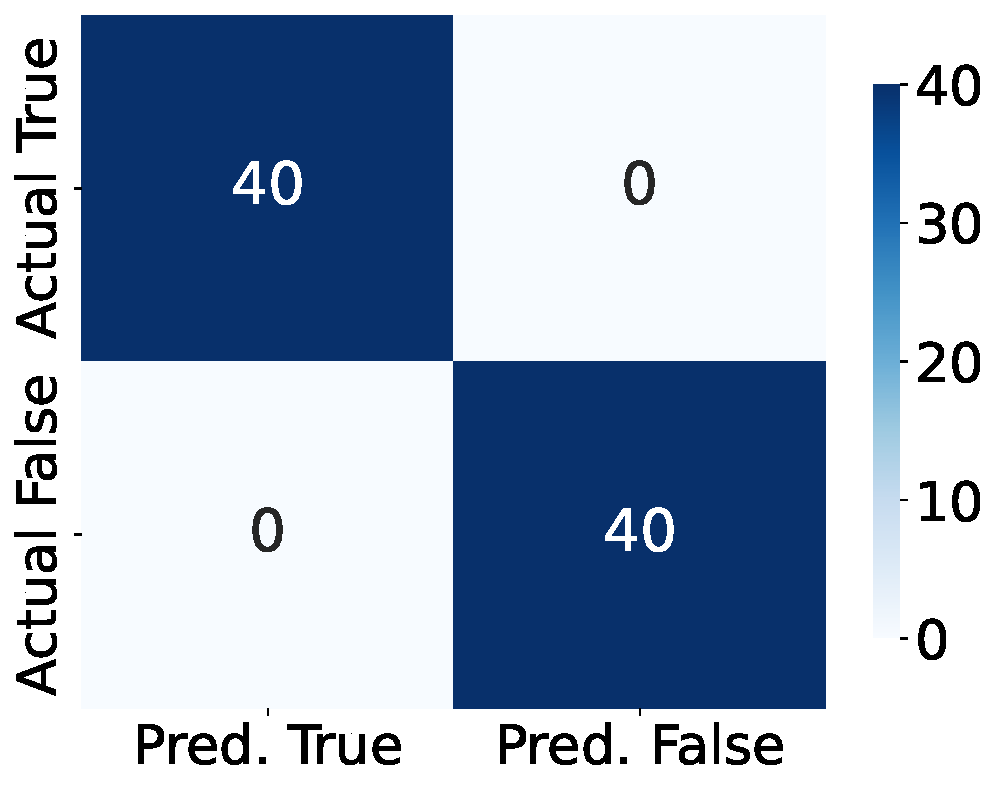
\includegraphics[width=\textwidth]{figs/confusion_matrix_answer_judge.pdf}
    \vspace{-5mm}
    \caption*{\tiny\shortstack{(a) Final answer}}
  \end{minipage}
  \hfill
  % subfigure 1
  \begin{minipage}[t]{0.19\textwidth}
    \centering
    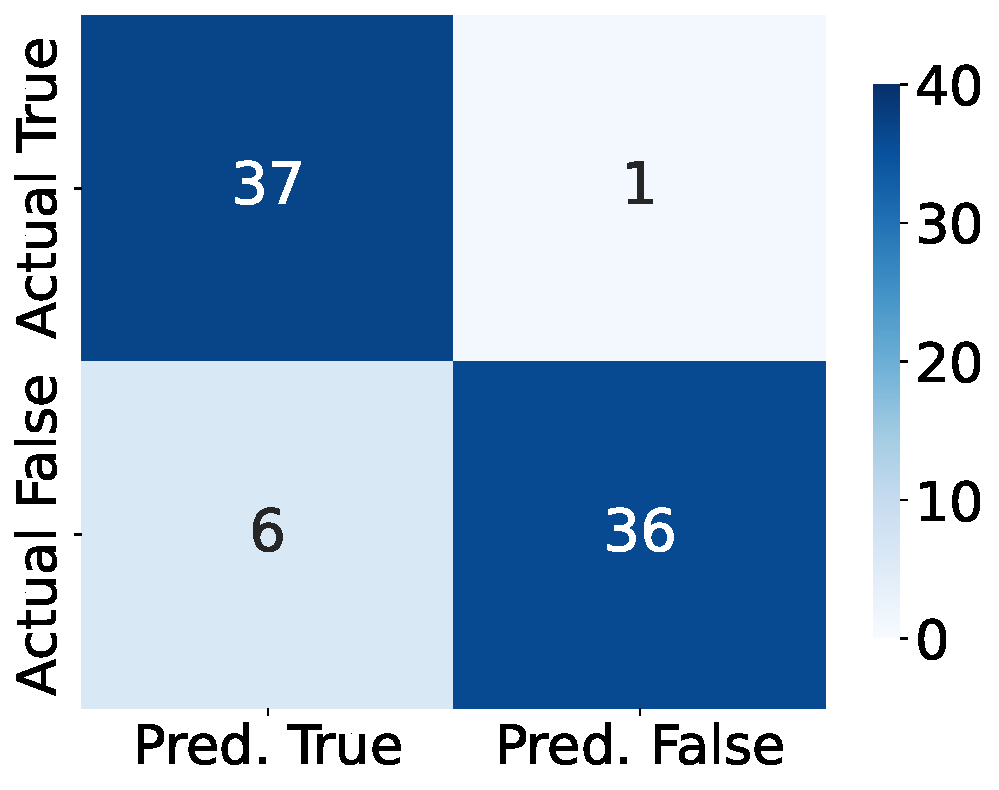
\includegraphics[width=\textwidth]{figs/confusion_matrix_toy_case_judge.pdf}
    \vspace{-5mm}
    \caption*{\tiny\shortstack{(b) Toy case}}
  \end{minipage}
  \hfill
  % subfigure 2
  \begin{minipage}[t]{0.19\textwidth}
    \centering
    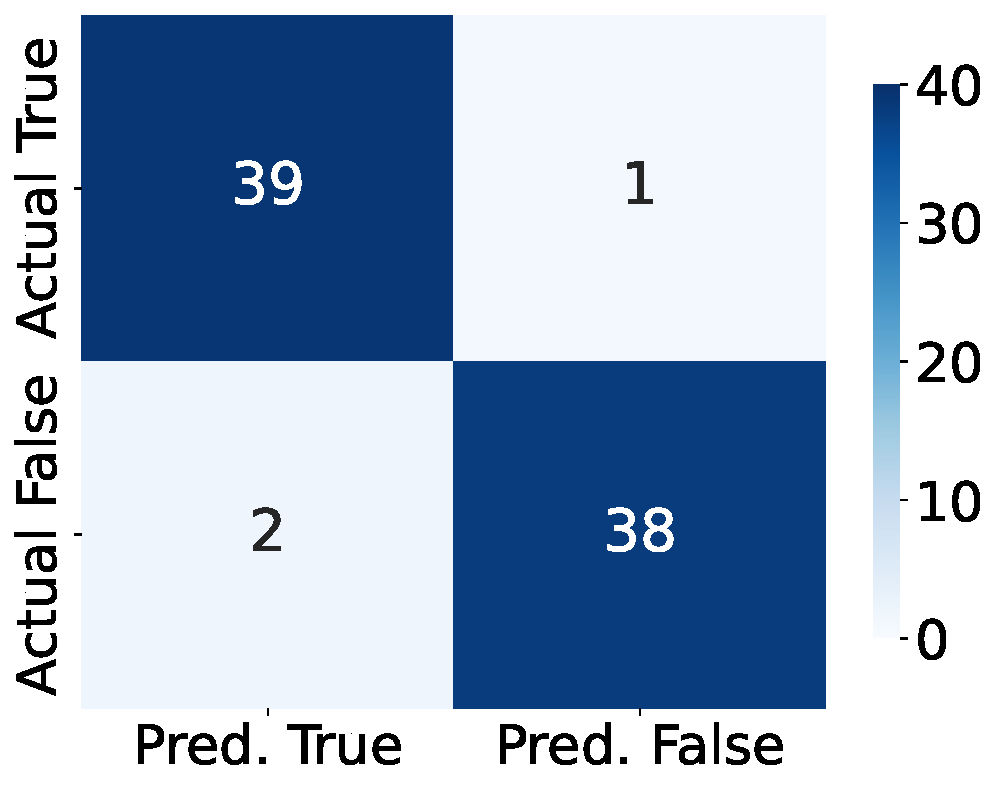
\includegraphics[width=\textwidth]{figs/confusion_matrix_logical_gap_judge.pdf}
    \vspace{-5mm}
    \caption*{\tiny\shortstack{(c) Logical gap}}
  \end{minipage}
  \hfill
  % subfigure 3
  \begin{minipage}[t]{0.19\textwidth}
    \centering
    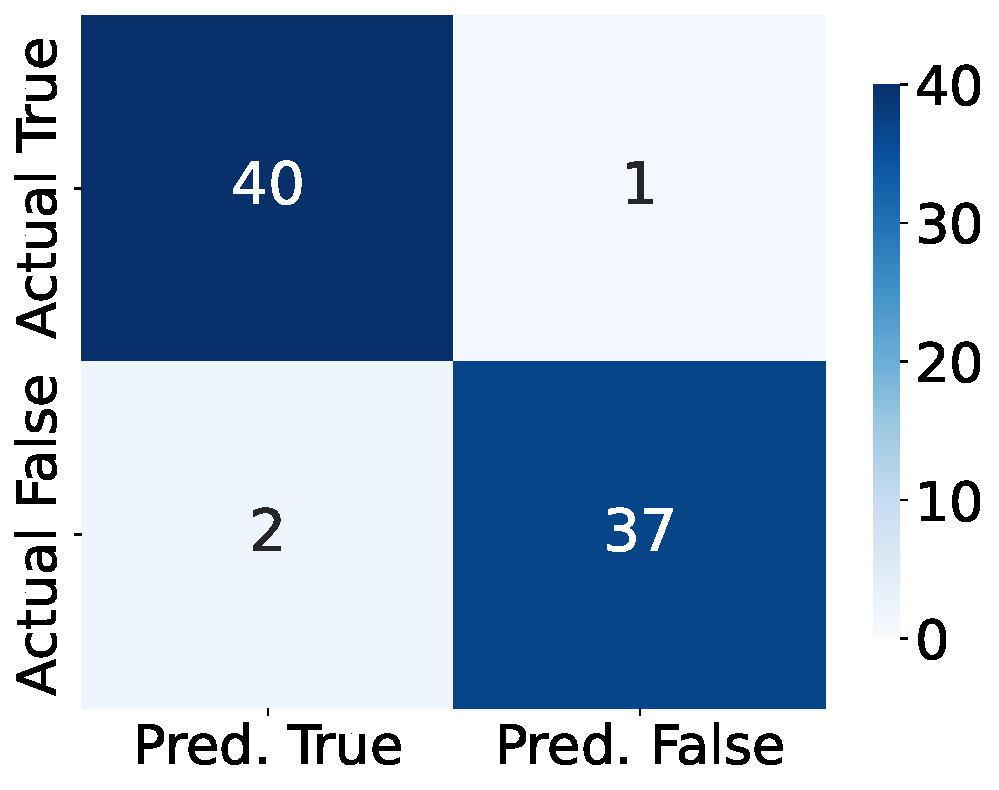
\includegraphics[width=\textwidth]{figs/confusion_matrix_approx_judge.pdf}
    \vspace{-5mm}
    \caption*{\tiny\shortstack{(d) Numerical approximation }}
  \end{minipage}
  \hfill
  % subfigure 4
  \begin{minipage}[t]{0.19\textwidth}
    \centering
    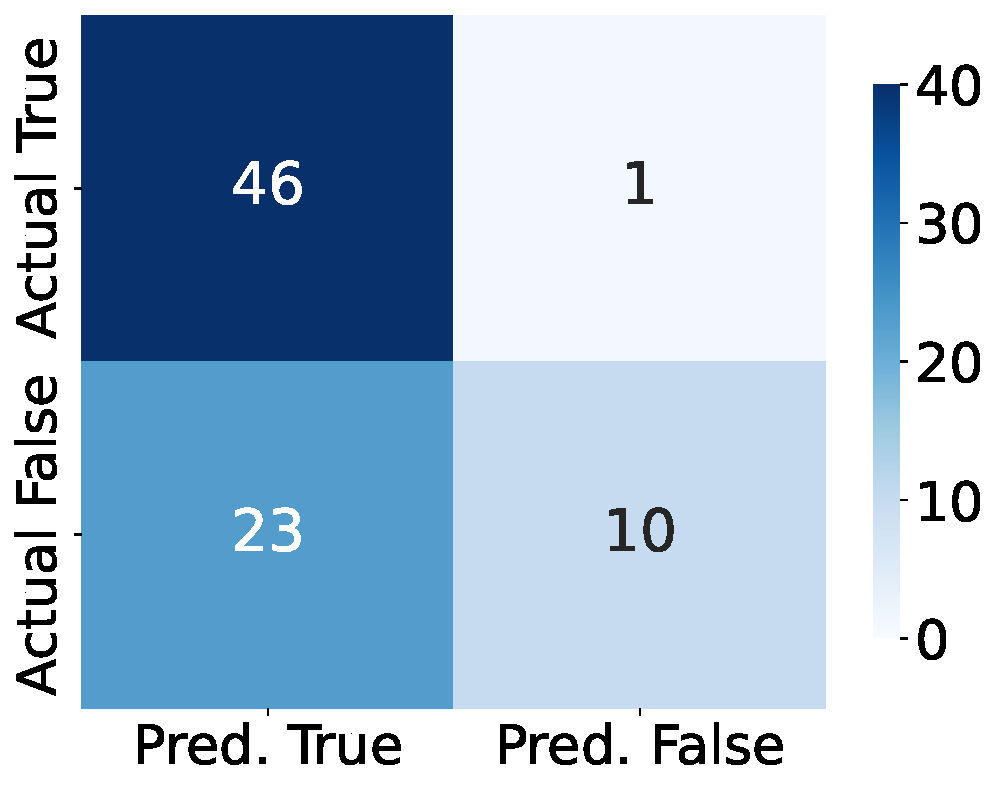
\includegraphics[width=\textwidth]{figs/confusion_matrix_calc_judge.pdf}
    \vspace{-5mm}
    \caption*{\tiny\shortstack{(e) Numerical computation}}
  \end{minipage}
  \vspace{-2mm}
  \caption{Confusion matrices for five judges, which exhibit strong agreement with human labels.}
  \vspace{-6mm}
  \label{fig:judge_confusion_matrix}
\end{figure}